\chapter{Le terminal virtuel}
C’est après l’apparition des ordinateurs personnels que les terminaux physiques ont cessé leur existence. Comme l’ordinateur était capable d’effectuer des calculs informatiques, il n'était plus nécessaire de recourir à des mainframes. Cependant, il restait indispensable de disposer d'une interface en ligne de commande pouvant lancer des commandes et communiquer avec le système d'exploitation. Pour remédier à cela, il fallait que l’ordinateur puisse \textit{simuler} un vrai terminal physique, c’est là que les terminaux virtuels ont vu le jour.

\section{La console virtuelle}
Historiquement, sur \textbf{UNIX}, le système d'exploitation avait un répertoire spécifique pour les terminaux physiques. Celui-ci se trouvait dans le répertoire \textbf{dev} et se nommait \textbf{ttySN} (où N correspondait au numéro du périphérique). Dorénavant les terminaux physique connecté via le port serie COM1 ne sont plus utiliser, mais à la place, c'est le répertoire \textbf{/dev/ttyN} qui est utiliser pour les terminaux virtuelles. Concernant les pseudo-terminaux que j'aborderai un peu plus bas, c'est le répertoire \textbf{/dev/pts/N}.
\newline

\begin{tcolorbox}[title=Pour information]
Par défaut, sur les distributions Linux, les consoles virtuelles sont au nombres de 64. Il y'a donc, au total 64 répertoires spéciaux \textbf{ttyN} (où N est de 0 à 63). Il est possible d'utiliser 8 consoles virtuelles en appuyant sur les touches \textit{CTRL+SHIFT+F1 à 8}.
\end{tcolorbox}

\newpage

\section{Le fonctionnement d'un terminal}
Le rôle principal d'un terminal est d'offrir une interface textuelle pour que l'utilisateur puisse interagir avec le système d'exploitation à travers des commandes. Il gère les entrées du clavier de l'utilisateur et également l'affichage des résultats des commandes à l'écran. Comme dit précédemment, en ce qui concerne les terminaux physiques, rien ne change dans leur fonctionnement, qu'ils soient physiques ou virtuels. Un terminal virtuel émule \footnote{Plus concrètement, cela signifie qu'il fonctionne comme s'il était un terminal physique.} tout simplement un terminal physique.

\subsection{Le répertoire spécial /dev}
Avant d'aborder plus en détail le fonctionnement d'un terminal, il faut d'abord comprendre ce que représente réellement le répertoire \textbf{/dev} et quel rapport il a avec les répertoires spéciaux \textbf{/dev/ttyN} mentionnés précédemment.

Sur Linux, on dit que \textit{tout est un fichier}. Ceci est totalement véridique, puisque lorsque un périphérique externe communique avec l'ordinateur, ce sont d'abord des signaux électriques qui sont transmis à l'ordinateur, et à partir de ces données, le système d'exploitation interprète ce qu'il reçoit. Par exemple, il existe un répertoire \textbf{/dev/input} qui permet de voir en temps réels ce qui se passe quand on appuie sur une touche ou bouge la souris. Dans le jargon de Linux, on appelle cela des 'event' ou 'évenement'.

\textit{Sans entrer plus en détail sur le fonctionnement des périphériques sur Linux, car ce sujet aborde exclusivement les terminaux et pseudo-terminaux. Un exemple explicatif court est donné sur la page suivante.}

Donc, le répertoire \textbf{/dev} est un répertoire spécial sur Linux qui joue le rôle d'interface pour les périphériques.

\clearpage

\begin{tcolorbox}[title=Pour information]
    Si l'on veut, par exemple, voir en temps réel les événements du clavier, il faut d'abord retrouver le fichier correspondant à l'événement du clavier, puis utiliser la commande \textit{cat} pour afficher le contenu du fichier.
    
    Il faut pouvoir récupérer le bon fichier \textit{event} qui représente le clavier : \textbf{cat /proc/bus/input/devices}

    \begin{verbatim}
    I: Bus=0011 Vendor=0001 Product=0001 Version=ab41
    N: Name="AT Translated Set 2 keyboard"
    P: Phys=isa0060/serio0/input0
    S: Sysfs=/devices/platform/i8042/serio0/input/input2
    U: Uniq=
    H: Handlers=sysrq kbd event2 % le n° de l'évenement
    B: PROP=0
    B: EV=120013
    B: KEY=4 2000000 3802078 f840d001 feffffdf f...
    B: MSC=10
    B: LED=7
    \end{verbatim}

	Par la suite, il faut juste afficher le contenu du fichier \textit{event} avec la commande \textit{cat}.
	C'est-à-dire, \textbf{sudo cat /dev/input/{N° de l'évenement} }
\end{tcolorbox}

\subsection{Les périphériques de type caractères et blocks}
Un dernier point à aborder est en rapport avec le répertoire \textbf{/dev/ttyN} : le type de périphérique attribué par le noyau. Il existe deux types de périphériques distincts sur Linux, les périphériques \textit{caractères} (ou character) et \textit{blocks}. La façon dont le noyau communique avec les périphériques dépend du type qui leur est attribué.

Pour être plus précis, c'est le pilote associé à un périphérique qui communique avec le noyau. Les pilotes dont les périphériques sont de types caractères vont envoyer et recevoir octet par octet. Contrairement aux pilotes dont les périphériques sont de types blocs qui envoient et reçoivent des blocs d'octets.

Les cartes son, terminaux, etc., sont des périphériques de type caractère, tandis que les disques durs, clés USB, etc., sont des périphériques de type bloc.

Les informations sur le type de périphériques peuvent être visibles dans la colonne \textit{type \& permissions} avec la commande \textbf{ls -l} :

\begin{verbatim}
Type & Permissions Liens  Propriétaire  Groupe  Majeur, Mineur  ...  Nom
crw-r--r--         1      root          root    10    , 235     ...   autofs
drwxr-xr-x         2      root          root    140             ...   block
...
\end{verbatim}

\newpage

Le fichier/répertoire peut avoir différents types. Voici une liste des types possibles :

\begin{itemize}
	\item \textbf{d} signifie que c'est un répertoire
	\item \textbf{l} signifie que le fichier est un lien symbolique
	\item \textbf{c} signifie que c'est un périphérique de type caractère
	\item \textbf{b} signifie que c'est un périphérique de type blocs
\end{itemize}

Comme mentionné plus haut, chaque périphérique possède un pilote qui lui est associé. Sans pilote, le périphérique ne peut pas recevoir ou envoyer des données au noyau, et vice-versa. Le pilote joue un rôle crucial pour la communication. Le terminal virtuel (\textit{/dev/ttyN}) possède aussi un terminal qu'on appelle \textbf{pilote de terminal}.

\subsection{Le pilote de terminal}
Le pilote de terminal joue un rôle crucial lors de l'utilisation des terminaux virtuels. Il gère deux tampons dans l'espace du noyau, lesquels sont en réalité des files recevant des données traitées par le pilote de terminal. L'un des tampons reçoit les entrées de l'utilisateur, appelé tampon \textbf{d'input}, tandis que l'autre reçoit les sorties du système, telles que la réponse à une commande entrée dans le shell, qui seront ensuite affichées sur l'écran. Toutes les entrées du clavier passent d'abord par le pilote du clavier. Sans entrer dans les détails du fonctionnement du pilote de clavier, une brève explication est fournie ci-dessus.

\begin{tcolorbox}[title=Une brève explication du pilote de clavier]
Tout périphérique possède un \textbf{pilote} qui lui est associé. Ce pilote joue un rôle important dans le bon fonctionnement du périphérique. Lorsqu'une personne appuie sur une touche du clavier, celui-ci envoie un '\textit{scan code}' directement à l'ordinateur. Chaque touche du clavier possède un '\textit{scan code}' bien précis, et c'est le \textbf{pilote du clavier} qui va transformer le \textit{scan code} en code ASCII compréhensible par le système d'exploitation. Pour chaque touche appuyée, une interruption est générée, et le \textbf{pilote du clavier} est informé qu'un \textit{scan code} doit être capturé.
\end{tcolorbox}

Le pilote peut être configuré en 2 modes différents :
\begin{itemize}
    \item \textbf{Mode canonique} : les données sont interprétées \textit{ligne par ligne}. Cela signifie qu'une ligne sera délimitée par un caractère spécial \textit{newline}. Le mode d'édition est activé, ce qui permet de modifier une ligne avant de la transmettre au tampon. De plus, les \textit{caractères spéciaux} sont pris en charge.
    \item \textbf{Mode non-canonique} : les données sont interprétées \textit{caractère par caractère}. Il n'y a pas de délimiteur comme pour le mode canonique. Certains \textit{caractères spéciaux} sont désactivés, ainsi que le mode d'édition.
\end{itemize}

\newpage

Quand le terminal est mis en mode canonique, il peut prendre en charge une multitude de caractères spéciaux. Certaines d'entre elles peuvent envoyer des signaux. Voici quelques-uns :

\begin{itemize}
	\item \textbf{INTR} : Ce caractère spécial permet de lancer un signal SIGINT à tous les processus en avant-plan qui détiennent le terminal de contrôle. Il peut être déclenché en utilisant la combinaison de touches \textit{CTRL+C}.
	\item \textbf{ERASE} : Ce caractère spécial permet de supprimer le dernier caractère inséré dans le tampon d'entrée. Il peut être activé en utilisant la touche \textit{BACKSPACE}.
	\item \textbf{EOF} : Ce caractère spécial permet de placer un délimiteur \textit{newline} à la fin du tampon d'entrée. Le pilote de terminal sera alors averti qu'il doit traiter toute la ligne jusqu'au délimiteur. Il peut être activé en utilisant la touche \textit{ENTER}.
\end{itemize}

Quand un terminal est utiliser, on s'aperçoit qu'il y a un \textbf{prompt} qui est affiché sur l'écran. Ce \textbf{prompt} est l'interpréteur de commandes, la plupart du temps il s'agit de \textit{bash}. En réalité, c'est un processus qui a été cloné et qui utilise le code de bash (en utilisant la commande \textit{exec}).

Ce programme est ce qu'on appelle un \textit{reading process}, un processus qui va \textit{lire le terminal}. Si le terminal est en mode canonique, les données stockées dans le tampon d'entrée seront lues par ligne. Une ligne est délimitée par un caractère spécial \textit{line feed} (voir plus haut). C'est seulement après le délimiteur que le shell va effectuer une demande de lecture au terminal pour récupérer ses données dans le tampon.

Une liste exhaustive de tous les caractères spéciaux est disponible sur Internet\footnote{\url{https://pubs.opengroup.org/onlinepubs/9699919799/basedefs/V1_chap11.html}}.

\begin{figure}[h]
	\centering
	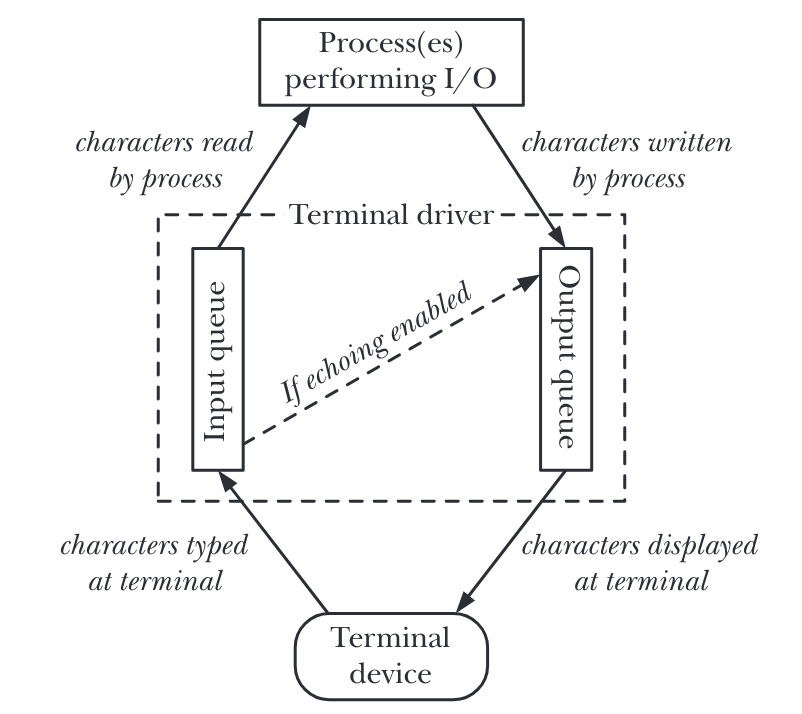
\includegraphics[width=250px, height=250px]{input_output_queue.png}
	\caption{Schéma montrant le tampon d'entrée et sortie dans le pilote de terminal}
\end{figure}

